\documentclass{llncs}

\usepackage{booktabs}
\usepackage{amssymb}
\usepackage{amsfonts}
\usepackage{graphicx}
\usepackage{url}
\usepackage{listings}
\usepackage{hyperref}
\usepackage{wrapfig}

\def\orcid#1{{\href{http://orcid.org/#1}{\protect\raisebox{-1.25pt}{\protect
\includegraphics{orcid.pdf}}}}}

\lstset{language=Python,showstringspaces=false}

\title{Learning Theorem Proving by Example - Implementing JavaRes (System Description)}

\author{Adam Pease\inst{1}\orcid{0000-0001-9772-1266}
        \and Stephan Schulz\inst{2}\orcid{0000-0001-6262-8555}
  }
\institute{
  Articulate Software, USA,
  \email{\tt apease@articulatesoftware.com}
  \and
  DHBW Stuttgart, Germany,
  \email{\tt schulz@eprover.org}
}


\titlerunning{Learning Theorem Proving by Example \emdash Implementing JavaRes (System Description)}

\renewcommand{\textfraction}{.01}
\renewcommand{\topfraction}{.99}

\newcommand{\mw}[1]{\ensuremath{\mathit{#1}}}
\newcommand{\nat}{\ensuremath{\mathbb N}}
\newcommand{\integer}{\ensuremath{\mathbb Z}}
\newcommand{\rat}{\ensuremath{\mathbb Q}}
\newcommand{\real}{\ensuremath{\mathbb R}}
\newcommand{\eqn}[2]{\ensuremath{#1\!\simeq\!#2}}
\newcommand{\neqn}[2]{\ensuremath{#1\!\not\simeq\!#2}}
\newcommand{\ueqn}[2]{\ensuremath{#1\dot{\simeq}#2}}

\newcommand{\limpl}{\rightarrow}
\newcommand{\limplies}{\rightarrow} % I mistype this too often ;-)
\newcommand{\ltrue}{\ensuremath{\top}}
\newcommand{\lfalse}{\ensuremath{\bot}}
\newcommand{\lequiv}{\ensuremath{\leftrightarrow}}

\newcommand{\terms}{\ensuremath{\mathit{Term(F,V)}}}
\newcommand{\tops}{\mathop{\mathrm{top}}\nolimits}
\newcommand{\pos}{\mathop{\mathrm{pos}}\nolimits}
\newcommand{\gfpf}{\mathop{\mathrm{gfpf}}\nolimits}
\newcommand{\fpf}{\mathop{\mathrm{fpf}}\nolimits}
\newcommand{\fp}{\mathop{\mathrm{fp}}\nolimits}
\newcommand{\text}[1] {\mbox{#1}}

\renewcommand{\textfraction}{.05}
\renewcommand{\topfraction}{.95}
\renewcommand{\bottomfraction}{.95}

\newcommand{\GInferenzC}[3]
{
\begin{tabular}{c}
  $#1$ \\
  \hline
  \raisebox{-0.4ex}{$#2$} \\
\end{tabular}
  #3
}

\newcommand{\CInferenz}[2]
{
\begin{tabular}{c}
  $#1$ \\
  \hline
  \hline
  \raisebox{-0.4ex}{$#2$} \\
\end{tabular}
}

%\pagestyle{empty}
%\bibliographystyle{alpha}
\bibliographystyle{splncs04}

\begin{document}

\maketitle


\begin{abstract}
  Did PyRes~\cite{SP:IJCAR-2020} achieve its goal of being a
  sufficient model for learning about how to implement a first-order
  ATP system?  JavaRes is a demonstration prover patterned after
  PyRes.  In this paper we discuss
  the architecture and data structures of this prover and the
  experience of one of us implementing the prover, without prior
  expertise in writing an FOL prover.  We provide performance metrics
  relative to PyRes.  To illustrate the
  value of JavaRes for learning about theorem proving we also mention
  implementation of several features beyond the original PyRes implementation.
\end{abstract}

\section{Introduction}

Automated theorem proving is a fascinating and useful discipline, but
can be mystifying for someone not deeply acquainted with the field.
It is fair to say that most computer science professionals do not
understand the power of inference in FOL and how it provides distinct
capabilities relative to simpler representations such as graphs or
description logics.  Part of the reason for this lack of general
familiarity may be because the barrier to entry in the field remains
high, despite many decades of work and publication.  Most publications
require a degree of mathematical sophistication to understand, and
even with such capability, a reader will not know which data
structures to use, or which of the many algorithms will be simplest or
best to implement.

We initially began with just an attempt for one of us (Pease) to learn
about automated Theorem Proving (ATP), motivated by decades of work in
formal ontology \cite{np01,p11}, and finding that among many excellent
books, including \cite{Harrison:HPL-2009}, the first steps to
understand ATP were too difficult.  Fortunately, the creator of the
prover \textbf{E}~\cite{Schulz:AICOM-2002,SCV:CADE-2019} (Schulz),
provided the explanations needed to understand how and where to begin.
This grew into the creation of PyRes.

PyRes is a simple, resolution-based theorem prover. It implements the
basic calculus from Robinson's seminal paper~\cite{Ro65}, extended
with negative literal selection and some redundancy elimination as
described by Bachmair and Ganziner~\cite{BG:HBAR-2001}. The core is a
given-clause based clausal saturation algorithm. The system also
supports full first-order input via clausification, and equality
handling via automatic addition of equality axioms.

%%% FIXME - the next sentence seems to be challenged grammatically,
%%% and I don't know what eactly you want to say.
To see whether PyRes provided
enough structure to learn how to write a theorem prover, we wrote
JavaRes and then used it as a platform to
implement several extensions.  We believe that the lessons learned
in the process, now incorporated into the two provers,
provide a suitable platform for ATP education.

JavaRes is open source and all code and data is available at
\url{https://github.com/ontologyportal/JavaRes}.




\section{Programming Language and Software Engineering Considerations}

Python is dynamically typed, which makes for flexible and fast
implementing, but also makes for a bit of a mismatch to Java, which is
statically typed.  The lack of static types can also cause confusion,
because the intended types are not documented at all points in the
code, since they are determined dynamically at runtime.  Java may hold
an advantage for education by requiring clarity in typing at compile
time.

Java, like Python, also provides call-by-value for simple data types
and call-by-reference for objects.  This is powerful, but also imposes
an obligation on the programmer to be mindful of side-effects in
methods.  It does allow for use of strategies such as shared term
rewriting, as in the C++ implementation of Eprover \cite{LS:LPAR-WS-2001}.

As a compiled language, Java also offers a speed advantage, which will
be evident when we show performance results comparing two provers that
use the same basic algorithms.

One lesson learned is that with code as complex as theorem proving
code, unless there is full understanding of the algorithm and expected
results, catching problems can be very challenging.  Minor coding
errors can be magnified since it is hard to know where to look in
system output for problems, and system output can be very large in a
combinatorially explosive search space.  Several such issues occurred
in the construction of JavaRes.  In one case literals were not
initialized as to whether literal selection had considered them
suitable for inference.  Copies were created of literals that included
their literal selection flag, rather than reinitializing them by
default as true.  This problem didn't cause any errors, just failure
to prove certain theorems (but not others) and therefore wasn't a
problem in simple examples and unit tests.  Another problem resulted
from a typo in subsumption where the variable 'subsumed' was mistyped
as 'subsumer'.  Even meaningful variable names can be a problem if
they are very similar to others.  A more serious case of a variable
naming issue that was present in a test case was having variables
named l1, ll and ll1 which could be easily confused in most fonts.

The process of creating PyRes and JavaRes was interrupted for several
years by the demands of other work and the challenge of coordinating
schedules between two busy people.  We started work on the project at
CADE in 2011 and mostly kept the Java and Python versions in sync,
working one day a week together for a period of a year.  Then there was a gap of 8 years and
a final push to bring JavaRes up to date with PyRes, consisting of two
months of half-time effort for one of us, plus occasional coaching and
some intensive debugging at the end.  This experience indicates that
implementing a basic prover patterned after PyRes should be feasible,
at least in terms of the time commitment involved, as a
graduate semester project after an introductory course in logic.

The code base of JavaRes is significantly more lines of code than
PyRes, in part due to Java being more verbose than Python, and in part
due to the implementation of analysis code in Java rather than in shell
scripts with PyRes, and also due to the implementation of additional
features and alternative algorithms.  JavaRes is 19,334 total lines of code vs 8553 lines
for PyRes (including comments, docstrings, and unit tests), and 7508 lines of effective
code for Java vs only 3681 lines of effective code for PyRes.  It is likely
that after this experience, refactoring and reimplementation could reduce
this discrepancy. However, code verbosity may be an advantage for educational purposes.

\section{Data Structure}

Figure \ref{fig:SysArch} shows the basic architecture of the system. A
subclass relationship is denoted by a hollow arrowhead.  A relationship
of one class (or instances of such a class) calling another is denoted
by a solid arrow.  One class that includes another in a member
variable is denoted by a hollow circle.  Each class is shown with its
name and at least some of its major methods.

JavaRes mirrors the data structures of PyRes.  At the bottom of the
hierarchy, \emph{terms} are built from variables (denoted in TPTP
syntax as an identifier with an initial capital letter, as in $X$ or
$Y$), constants (denoted by an initial lowercase as in $a$ or $b$) and
function symbols, which allow nesting (as in $p(X)$ and $g(f(a))$),
\emph{Atoms} are built from predicate symbols and term arguments, like
$partOf(myWheel,myCar)$.  Note that once we handle equality, $=$ is
allowed as an infix predicate symbol. While predicate symbols and
function symbols, as well as terms and atoms, share the same internal
representation, \emph{literals}, which are possibly negated atoms,
have their own distinct representation. Literals are combined in lists
to buld \emph{clauses}, which are interpreted as disjunctions of
literals and represented by a distinct class which also includes
meta-data.  Until this point, the only logical operators considered
are equality, negation and disjunction (logical 'or').

All these components have methods for printing themselves, parsing
from both TPTP and SUO-KIF, using the \emph{Lexer} class, creating a new
copy, testing for equality and sort order. Of the classes mentioned so
far, only terms, literals, and clauses are actually used in proof
seach.  \emph{Formulas} are parsed and converted to CNF.  JavaRes has
two clausifiers: \emph{Clausifier} implements the classical algorithm
from \cite{RN:AI-95} and \emph{SmallCNF}, which includes miniscoping
and simplification as described by Nonnengart and
Weidenbach~\cite{NW:SmallCNF-2001}.

To hold a set of clauses the prover is working on, we also have the
class \emph{ClauseSet}.

\begin{figure}
  \centering
  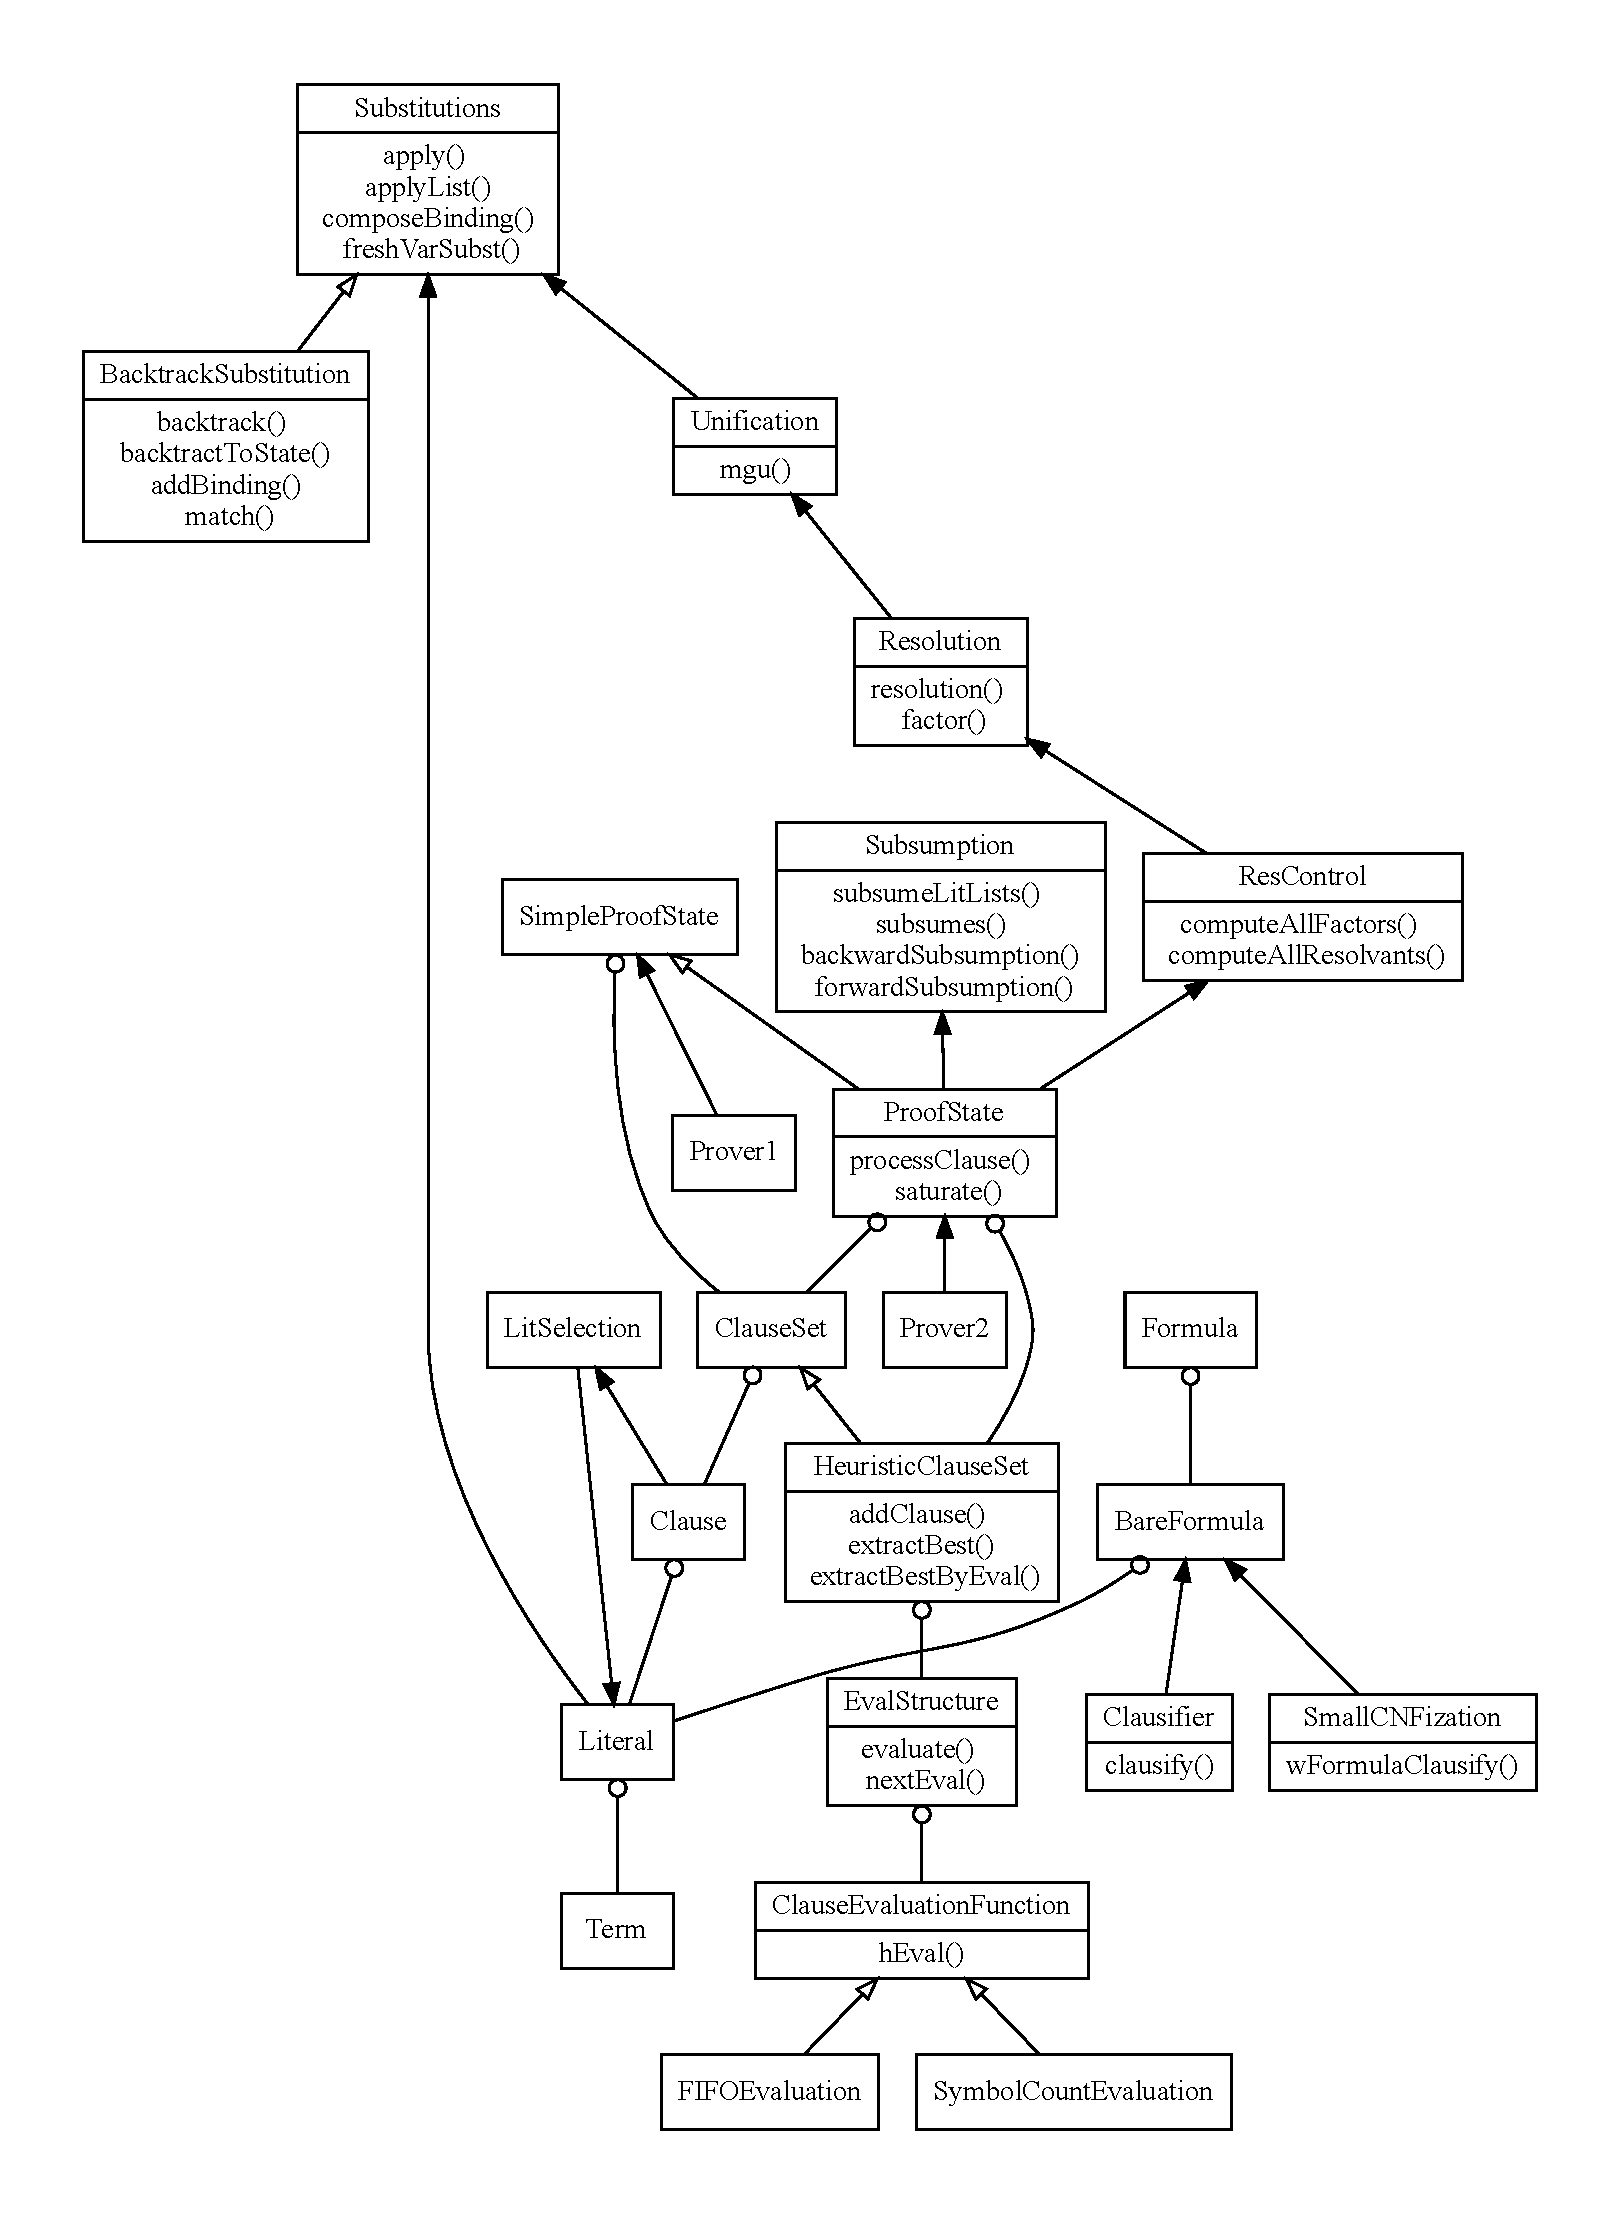
\includegraphics[width=6in]{architecture.pdf}
  \caption{Basic System Class Diagram}
  \label{fig:SysArch}
\end{figure}

\section{Class Structure}

Several classes implement the machinery of proving.  The most
fundamental is that of \emph{Substitution}, which replaces variables with
\emph{Term}s (including other variables).  The class \emph{Unification} attempts to
unify the structure of two lists of \emph{Term}s and results in a set of
\emph{Substitution}s.  \emph{Substitution}s are also created when we rename
variables in clauses to ensure that variables in different clauses,
which are logically different, also have syntactically different
names.  The class \emph{Resolution} iterates through \emph{Literal}s in a given pair
of \emph{Clause}s, attempting to find unifiable literals with opposite signs.
\emph{Resolution} also handles factoring, in which a \emph{Clause} is simplified
when one of its \emph{Literal}s unifies with another, thereby enabling
removal of the more specific \emph{Literal}, applying the resulting
\emph{Substitution} to all remaining \emph{Literal}s.  The class \emph{ResControl} is
simple, finding all factors within a given \emph{Clause}, and all resolvants
between a given \emph{Clause} and \emph{ClauseSet}.  The class \emph{SimpleProofState}
keeps a set of \emph{Clause}s that have already been processed, which is
subjected to resolution and factoring, and those \emph{Clause}s that have not
yet been processed.  Its primary method, \texttt{saturate()}, keeps calling its
\texttt{processClause()} method, picking an arbitrary unprocessed \emph{Clause} for
resolution and factoring, and continuing until a contradiction is
found or there are no more unprocessed clauses to try.  The class
\emph{Prover1} is the top level of our simple prover.  It simply calls
\emph{SimpleProofState} reads in a \emph{ClauseSet}.

\section{Improvements}

We improve on the SimpleProofState class with \emph{ProofState}. It performs
several functions.  In addition to saturation, it also holds the state
of various options and heuristics for the provers, which we will
explain shortly, and the derivation of a proof by contradiction,
consisting of relationships among \emph{Clause}s that detail how they were
derived from the originally given \emph{Clause}s.

We also add above \emph{Clause} the class \emph{BareFormula}, which can have
logical operators (such as quantification, implication, equivalence,
and conjunction, as well as less common operators such as
`$<\thicksim>$').  We have formula wrappers, in the class \emph{Formula},
that include the data seen in TPTP problems, such as the type of the
statement ('cnf', 'fof', 'thf' etc), the formula name and the type of
the formula ('conjecture', 'plain' etc) as well as other data that is
determined and used during ATP. In order to convert \emph{Formula}s into
C\emph{lause}s, we have the classes \emph{Clausify} and \emph{SmallCNFization}, which
implement two different algorithms for conversion to conjunctive normal
form.

We implement the class \emph{Prover2} in order to support reading TPTP or
SUO-KIF formulas and converting them to CNF before saturation.
Prover2 also has routines to handle setting options and returning
proofs.  The new \emph{ProofState} class uses a topological sort
\cite{DBLP:journals/cacm/Kahn62} to create a linearized proof in TSTP
format from the proof graph.  It also outputs dot format to supporting
rendering of a proof graph by GraphViz\footnote{\url{https://graphviz.org/}}.
In addition, JavaRes employs an
algorithm for answer extraction that attempts to search in a proof from
a conjecture with an existentially quantified variable to a supporting
clause that contains a binding for that variable.  This is a very useful
feature in practice as it allows a user to get answers to logically
formulated questions, rather than just \texttt{\$true} or \texttt{\$false}.

\subsection{Clause Selection, Indexing, Heuristics, SInE and other Features}

JavaRes includes all the optimization strategies in PyRes.  For clause
selection it implements two methods, which can be combined.  The most
basic is a first-in-first-out (FIFO) strategy that will eventually try every
clause.  However, this is rarely optimal.  A symbol-counting strategy
picks the clause with the fewest symbols.  This is often a good
strategy but in many cases it will fail because larger clauses may
never be considered.  The most successful simple strategy turns out to
be a combination of the two, where the smallest symbol count is tried
five times and then FIFO is tried once.  This results in a strong bias
to smaller clauses while ensuring that all clauses will eventually be
tried.  JavaRes also supports a more conservative stregy of two tries
with the smallest symbol for every one try of the FIFO stack.  Other
combinations are possible with a small change to the code.

JavaRes supports indexing for subsumption and resolution.  Subsumption
removes clauses from the set of clauses to be processed (called
``forward subsumption'') and from the set already processed (``backwards
subsumption'') thereby decreasing the problem search space.  More
general clauses subsume more specific ones.

Indexing employs
records with signs and predicate symbols only, so that potential clauses can
be accepted or rejected more rapidly than attempting unification.  In resolution, literals of opposite sign may resolve,
as opposed to subsumption in which those of the same sign potentially subsume.
Resolution and subsumption therefore have separate indexes.

JavaRes also implements PyRes' approach to literal selection.  A naive
approach to resolution has to compare every literal in a resolver to
every literal in the proposed resolvant to see if they unify but have
opposite signs.  Optimizations other than this exhaustive approach can
have an impact.  We implement five strategies: choose simply the first
literal, the largest literal, the smallest number of constants and
variables, the smallest number of variables and finally, a combined
strategy that picks an equation of two variables, if present, or the
smallest number of variables or if those are equal then the largest
number of symbols.  Largest literal selection is the default strategy.

For large theories, JavaRes has implemented the SInE
algorithm\cite{HV:CADE-2011} that has proven to be the dominant approach in the
LTB division of the CASC competition.

JavaRes can also parse the first order portion of SUO-KIF syntax used
with the SUMO knowledge base that is arguably a much more friendly
syntax for theory authoring, especially for complex or nested axioms,
than TPTP.  The JavaRes data structures used for ATP with the different surface
syntax of SUMO are identical with TPTP.

An additional utility that JavaRes supports is creation of proof
graphs intended to be visualized with the GraphViz renderer.

\section{Testing and Examples}

It is very valuable to have many examples.  When examples are
implemented as unit tests they catch bugs as well as explain how the
algorithms are supposed to work at each stage.  The example provide a
sense of purpose for each class, and are as valuable as the algorithms
themselves.  Often, just having a clear set of examples is sufficient
to code at least some version of the algorithm needed.  Adding more
tests and examples has been a key benefit of the implementation of
JavaRes, as it showed what obscure bugs might appear, or what
non-obvious errors might exist.  For example, in an early version of
unification, the implementation failed to consider all possible
options, just returning a list of one set of substitutions, rather
than all possible substitution.  This problem didn't surface in
testing until much later, but was easily explained with an example and
test that should ensure that no future implementer will move forward
with an implementation while being unaware of this issue, should it
arise.  Java tests are implemented in the jUnit framework.  Whereas
Python coders add tests at the end of each class, in Java tests are
separated into their own classes.

One of the lessons from implementing JavaRes is that one can never
have too many tests.  A number of bugs, mostly from typographical
errors, were not evident in the unit tests and only appeared once
tested on some of the larger problems in the TPTP.  Even smaller TPTP
problems could lead to false confidence, since several successful
paths to a contradiction often exist and only on problems that are
challenging will the absence of a particular component of proving,
such as forward subsumption, be a critical issue.



We present the results in Table \ref{tab:res} for different problem
classes within TPTP: UEQ (unit problems with equality), CNE (clausal
problems without equality), CEQ (clausal problem with equality, but
excluding UEQ), FNE (FOF problems without equality) and FEQ (FOF
problems with equality).  Readers interested in performance of the
systems in other than their best configuration can refer to our
previous PyRes paper and we only present the systems here with their
performance including indexing, subsumption and best clause selection
strategy.

As with our earlier experiments with PyRes, testing was on StarExec
Miami, a spin-off of the original StarExec project
\cite{SST:IJCAR-2014}. StarExec proved to be an essential resource for
scaling up testing as it is not practical to run all
\textasciitilde24,000 available tests for 300 seconds each on a
laptop, or to load it so heavily with theorem proving that no other
work can be done.  Even so, running an experiment of this sort can
take 24 hours of clock time, unless there is no other load on the
system. It was tempting, too early in the development process, to run
the full set of TPTP tests.  After several abortive attempts, a much
smaller set of problem tests was used to create an integration test
suite that was more comprehensive that unit tests, nearly as fast, and
certainly much faster than an indiscriminate run on all available TPTP
problems.

The StarExec machines were equipped with 256 GB of RAM and Intel Xeon
CPUs running at 3.20 GHz.  The per-problem time-limit was set to 300
seconds. TPTP 7.4 was used but only on problems also present in 7.2,
to allow for continuity with the measurements in our earlier paper on
PyRes.

JavaRes begins to approach the performance of Prover9 on problems without
equality.  Implementing the JavaRes/PyRes approach to ATP
in C or C++ would likely result in further speed improvements.

\begin{table}[tbh]
  \begin{tabular}{lrrrrrr}
    \hline
    \textbf{Category} & \textbf{UEQ} & \textbf{CNE} & \textbf{CEQ} & \textbf{FNE} & \textbf{FEQ} & \textbf{All}\\
    {\tiny Class size} & {\tiny (1193)} & {\tiny (2383)} & {\tiny (4442)} & {\tiny (1771)} & {\tiny (6305)} & {\tiny (16094)}\\
    \hline
    PyRes              &   113 &  945 &   499 &   632 &   725 &  2914 \\
    JavaRes            &   173 & 1081 &   615 &   737 &  1589 &  4195 \\
    \hline
    E 2.4              &   813 &  1939 &  2648 &  1484 &  4054 & 10938 \\
    Prover9-1109a      &   728 &  1316 &  1678 &   709 &  2001 &  6432 \\
    LeanCoP 2.2        &     6 &     0 &     0 &   969 &  1826 &  2801 \\
    \hline
  \end{tabular}
  \caption{JavaRes and PyRes problem correctness (E, Prover9 and leanCoP for comparison)}
  \label{tab:res}
\end{table}

We also looked at computation time since many successful problems finish in significantly less than the allotted
300s limit.  Failed problems were assessed 300s so we could get a comprehensive metric without giving credit
for cases where the theorem prover just gave up or timed out.  For each category we present to total minutes of computation time for all
the TPTP problems in the given category (Table \ref{tab:res2}). However because so many test problems fail with these
relatively basic provers, the speed difference is somewhat obscured.

\begin{table}[tbh]
  \begin{tabular}{lrrrrrr}
    \hline
    \textbf{Category} & \textbf{UEQ} & \textbf{CNE} & \textbf{CEQ} & \textbf{FNE} & \textbf{FEQ} & \textbf{All}\\
    \hline
    PyRes              &   5457 &  7395 &   19929 &   5800 &   28193 &  66777 \\
    JavaRes            &   5171 &  6618 &   19326 &   5231 &   23681 &  60028 \\
    \hline
  \end{tabular}
  \caption{JavaRes and PyRes total TPTP suite execution time in minutes}
  \label{tab:res2}
\end{table}

We also compare just those problems that were solved by both provers in order to better show execution speed,
and the difference is then more evident (Figure \ref{tab:res3}).

\begin{table}[tbh]
  \begin{tabular}{lrrrrrr}
    \hline
    \textbf{Category} & \textbf{UEQ} & \textbf{CNE} & \textbf{CEQ} & \textbf{FNE} & \textbf{FEQ} & \textbf{All}\\
    \hline
    PyRes     &   57 &  169 &   189 &   89 &   121 &  628 \\
    JavaRes   &   7 &   28 &   30 &   32 &   32 &  131 \\
    \hline
  \end{tabular}
  \caption{JavaRes and PyRes TPTP suite successful-only execution time in minutes}
  \label{tab:res3}
\end{table}


The problems on which JavaRes and PyRes differ appear to be where the timeout limit is just beyond
the reach of PyRes.  For example TPTP problem LCL858-1.p is solved in 86 seconds by JavaRes while
PyRes fails to find the answer in 300 seconds.  But given more time, PyRes finds the answer in 508 seconds.
In total, JavaRes solves 1321 problems within the time limit that PyRes does not.  However, PyRes also
solves 180 problems that JavaRes does not.


\section{Conclusion and Future Work}

The experience of JavaRes has shown that it is possible to use PyRes
as the basis for a new theorem prover implementation in about three
person months of work, albeit with some coaching, and for someone
already familiar with TPTP, as a user of TPTP and with FOL generally.
The experience has shown us how to improve the clarity of the code,
and expand code comments and unit tests.

With an implementation in Java, it should be easier to integrate the
prover with existing tools to support special cases that apply to SUMO
development, since its existing Sigma tool set \cite{pease2013sigma}
and SUMOjEdit editor \cite{pease2020programmer} are also written in
Java.  Having a testbed for theorem prover features enables creating
proof-of-concept implementations that may then transfer to a
higher-performance implementation, such as E.  One such possibility is
to include a pluggable interface for external functions.  These could
be as simple as arithmetic functions or as complex as calls to
databases, such as in \cite{DBLP:conf/ki/SudaSWLM09}.  Also of
interest would be an implementation of a "Why-Not" function
\cite{10.5555/1650083.1650093} that could guide the commensense theory
developer in filling gaps in proposed inference paths.

\section{Acknowledgements}

Thanks to Geoff Sutcliffe for his work on, and advice about, StarExec
and TPTP, which allowed us to test our work.

% ORCID for Adam Pease - \footnote{\url{https://orcid.org/0000-0001-9772-1266}},
% Stephan Schulz \footnote{\url{https://orcid.org/0000-0001-6262-8555}}.

\bibliography{stsbib}
\end{document}

%%% Local Variables:
%%% mode: latex
%%% eval: (tex-pdf-mode)
%%% TeX-master: t
%%% End:
